\documentclass{sig-alternate}
\usepackage{etoolbox}
\makeatletter
\patchcmd{\maketitle}{\@copyrightspace}{}{}{}
\makeatother
\usepackage{amsmath,amssymb,graphicx}
\usepackage[ruled,linesnumbered]{algorithm2e}
\usepackage{algorithmic}
\usepackage{tablefootnote}
\usepackage{slashbox}
\usepackage{siunitx}
\usepackage{threeparttable}
\usepackage[hidelinks]{hyperref}
\usepackage{epstopdf}
\newcolumntype{C}[1]{>{\centering\let\newline\\\arraybackslash\hspace{0pt}}m{#1}}
\newcommand{\suchthat}{\, \mid \,} 
\DeclareMathOperator*{\argmin}{argmin}
\DeclareMathOperator*{\argmax}{argmax}
\usepackage{url}

\usepackage{natbib}
\setlength{\bibsep}{0pt plus 0.3ex}
\usepackage{kantlipsum}
\makeatletter
\def\@maketitle{\newpage
 \null
 \setbox\@acmtitlebox\vbox{%
\baselineskip 20pt
\vskip 2em                   % Vertical space above title.
   \begin{center}
    {\ttlfnt \@title\par}       % Title set in 18pt Helvetica (Arial) bold size.
    \vskip 1.5em                % Vertical space after title.
%This should be the subtitle.
{\subttlfnt \the\subtitletext\par}\vskip 1.25em%\fi
    {\baselineskip 16pt\aufnt   % each author set in \12 pt Arial, in a
     \lineskip .5em             % tabular environment
     \begin{tabular}[t]{c}\@author
     \end{tabular}\par}
    \vskip 1.5em               % Vertical space after author.
   \end{center}}
 \dimen0=\ht\@acmtitlebox
% \advance\dimen0 by -12.75pc\relax % comment by Marco Daniel
 \unvbox\@acmtitlebox
 \ifdim\dimen0<0.0pt\relax\vskip-\dimen0\fi}
\makeatother

\usepackage[T1]{fontenc}
\usepackage{lmodern}
\title{A Comparison of Antenna Placement Algorithms}
\author{\alignauthor
    Abhinav Jauhri\\
    \affaddr{Carnegie Mellon University}\\
\email{ajauhri@cmu.edu}}
\begin{document}
\maketitle
\begin{abstract}
Co-location of multiple antenna systems on a single fixed or mobile platform can be challenging due to a variety of factors, such as mutual coupling, individual antenna constraints, multipath, obstructions, and parasitic effects due to the platform. The situation frequently arises where a new communication capability, and hence antenna system, is needed on an existing platform. The problem of placing new antennas requires a long, manual effort in order to complete an antenna placement study. An automated procedure for determining such placements would not only save time, but would be able to optimize the performance of all co-located antenna systems. In this paper we examine a set of stochastic algorithms to determine their effectiveness at finding optimal placements for multiple antennas on a platform. To our knowledge, this is the first study to investigate optimizing multiple antenna placement on a single platform using multiple stochastic algorithms. Of the four algorithms compared on the basis of convergence rates, simulated annealing and evolutionary strategy were found to be most effective in finding optimal placements.
\end{abstract}
% A category with the (minimum) three required fields

\section{Introduction}
Antenna placement on a multi-antenna platform currently involves a manual process that is challenging, time-consuming, and may result in sub-optimal placements leading to lowered communication systems' performance. Moreover, the search space becomes exponentially large with regard to the number of antennas to be placed ($|\text{search space}| = m^n$, where $m$ is the number of allowable placements for each antenna and $n$ is number of antennas). 

Applying an evolutionary algorithm (EA) to this problem could greatly improve this process by automatically determining acceptable antenna placements.  Evolutionary algorithms encompass a variety of computer search technologies, with the Genetic Algorithm (GA) being the most well-known \cite{holland1975adaptation}. EAs have proven very capable in discovering high performance antenna designs and previous work has been responsible for a number of advances \cite{haupt2007genetic}, including the seminal patent for this process and genetically-evolved antennas deployed in space \cite{linden1997automated, lohn2005evolutionary}.  Additionally, our work is \textit{highly generic} such that any type of a platform may be used to find optimal placement of antennas.

Our main contributions are:
\begin{itemize}
    \item Applying existing stochastic algorithms to help determining optimal or near-optimal antenna placements on a platform
    \item Our approach is agnostic of the type of platform used
    \item We apply experiments on different types of platforms and antennas to demonstrate the effectiveness of different stochastic algorithms
\end{itemize}

\section{Related Works}
\label{sec:related}
The problem of optimizing the placement of multiple antennas on a single platform has rarely been studied, if at all.  The closest research we have found concerns algorithms for locating and configuring infrastructure  for cellular wireless networks with the assumption of isotropic radiation pattern.  Another related is work used characteristic mode analysis to compute optimal antenna locations for an antenna placed within a mobile device \cite{famdie2007optimal}. In our work, none of the algorithms discussed have prior information of good antenna placements or type of antennas to be placed on the platform.

In addition, the related problem of co-designing antennas for a given platform ({\em in-situ} design) using EAs has been investigated in \cite{linden2000wire} with encouraging results. Because antenna placement bears many similarities to antenna design, we believe that such algorithms will prove effective.

\section{Problem Formulation}
\label{sec:problem}
A platform for our problem formulation could vary from a simple rectangular box to an aircraft. 
\subsection{Inputs}
\label{sec:inputs}
Our inputs to an algorithm shall comprise of a platform and set of antennas each with allowable placements on the platform. Formally, a platform, $P$, in 3-dimensional space with its surface discretized into a regular grid with some spacing consisting of potential antenna placement points (see Figure \ref{fig:plat1}). Let $m$ denote the number of antennas to be placed on $P$ such that $m>1$, and let $A$ represent the set of antennas: $A = \{A_1, ..., A_m\}$.  For each antenna $A_i$, let $L_i$ denote the set allowable placement coordinates $\in \mathbb R^3$ on $P$ such that $\mid L_i \mid =n_i$, and $ \forall i, n_i>1$:
\[
L_i = \{(x_{1}, y_{1}, z_{1}), ..., (x_{n_i}, y_{n_i}, z_{n_i})\}
\]


\begin{figure}
    \begin{center}
        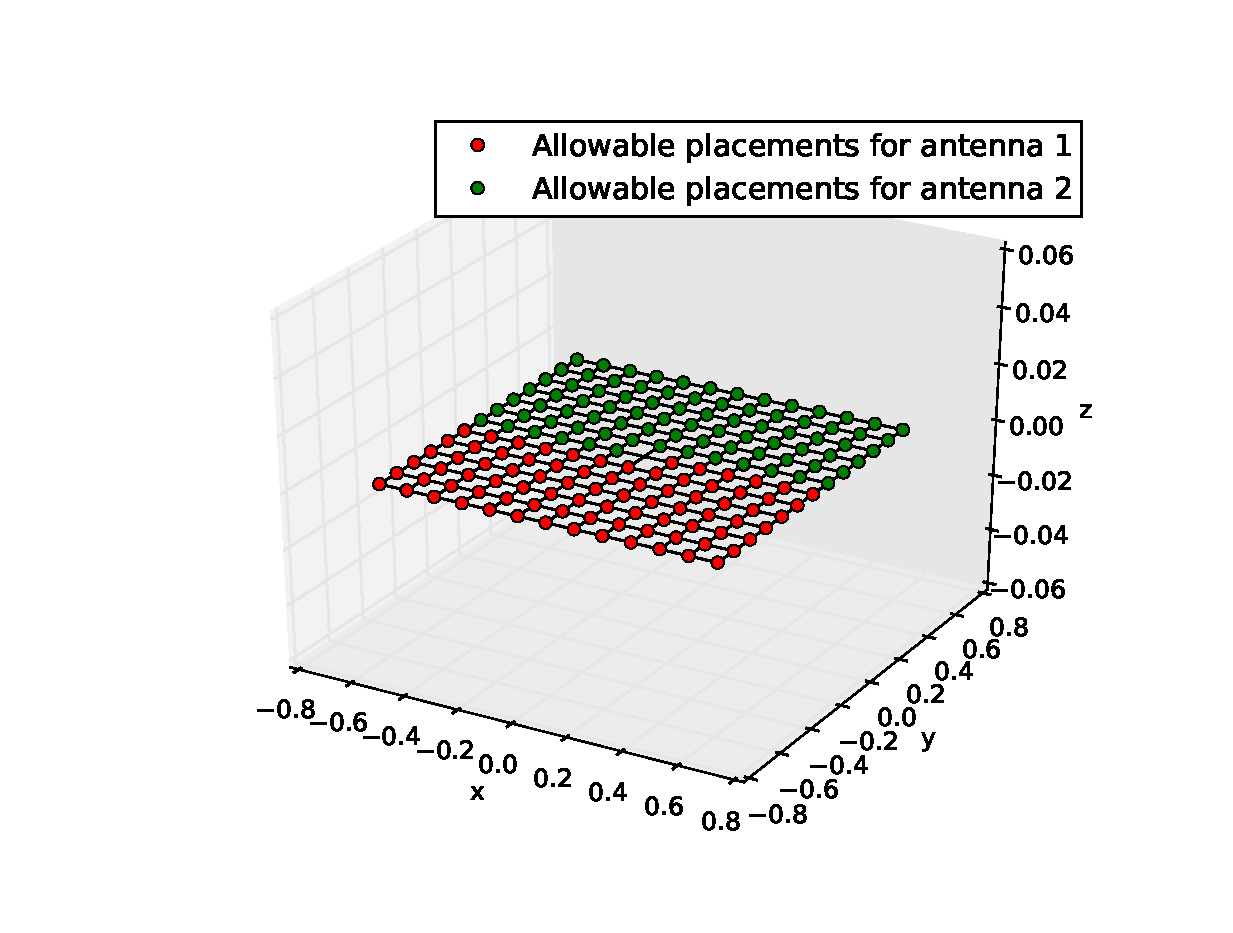
\includegraphics[width=.41\textwidth]{FIG/tc_1_figure}
\end{center}
\caption{Platform used for test case 1 (tc1) \& 4 (tc4)}
\label{fig:plat1}
\end{figure}

Using the inputs, a \textit{candidate solution/individual}, $H$, is formed by a set of $m$ antenna locations. In other words, a hypothesis is a placement configuration i.e. a set having $m$ placements, one for each of the $m$ antennas, in 3-dimensional space:
\[
    H  = \left\{(x_1, y_1, z_1), \cdots, (x_m, y_m, z_m)\right\}
\]

The reader should note that the number of allowable placements for any antenna are finite. We shall elaborate how that is ensured later in Section \ref{sec:setup}.

\subsection{Fitness Evaluation}
The placement optimization aims to find the best \textit{hypothesis}, $H^*$, such that the radiation pattern and mutual coupling are optimal. For optimal radiation pattern, we shall minimize the difference between the free-space gain pattern (FSG) of antenna $A_i$, and its pattern when placed on $P$ and in the presence of all remaining antennas (in-situ gain, or ISG).  Thus, for each gain point for $A_i$ we compute:

\begin{equation} \label{eq:rp}
  F_{RP}(A_i) = \sum_{\theta}\sum_{\phi} 
           \| ISG_i(\theta,\phi) - FSG_i(\theta,\phi) \| ^2,
\end{equation}

where $\theta$ \& $\phi$ define the spherical and cylindrical coordinates of a field point respectively (see \textit{Section 5 for more information}).

For the second objective, it is desired to minimize the mutual coupling between the antennas for a given placement configuration because strong mutual coupling reduces antenna efficiency. This is computed in a pairwise manner where the CP function computes the coupling between two antennas:
\begin{equation}
  F_{MC} = \sum_{i=1}^{m-1}\sum_{j=i+1}^{m} CP(A_i, A_j)
\end{equation}

The overall optimization for a given placement configuration is to minimize fitness, $F$, as follows optimal antenna placement for mobile terminals using characteristic analysis:
\begin{equation} \label{eq:optimal}
  F = \alpha F_{MC} + \beta \sum_{i} F_{RP}(A_i),
\end{equation}
where $\alpha$ and $\beta$ are constants which satisfy: $\alpha + \beta = 1$. $F$ will be provided by an antenna simulation software which will be introduced in Section \ref{sec:setup}.

Radiation pattern and antenna coupling are measured in decibels (dB) which is a logarithmic unit used to express the ratio between two quantities i.e. $10 \cdot \log{x_1 / x_2}$. For radiation pattern fitness parameter, the \textit{antenna strength} or gain shown in Eq.\eqref{eq:rp}, at any given point on a sphere is the ratio of the signal strength of the antenna being tested to a perfectly isotropic antenna, expressed in dB. For coupling, the ratio compares the energy absorbed by one antenna when the another antenna is operating nearby.  For our antenna placement problem, this absorption is undesirable because we want the energy to be radiated away in order to establish a communication link, and not be absorbed by a nearby antenna.  This coupling thus reduces the antenna's efficiency.  For example, if the coupling ($F_{MC}$) was $-10$ dB for an hypothesis instead of the best, let's say $-13$ dB, then this reflects a difference $\Delta_c$ of $3$ dB which translates to a doubling of energy absorbed in the -10 dB case compared to the -13 dB case. Shown in Table \ref{tab:importance} is the equivalence of overall fitness ($F$) to $\Delta_c$. Also shown is the equivalence to expected gain defined as:
\begin{equation}
    \mathbb E_g = \frac{1}{N \cdot m} \sum_{i}^m F_{RP}(A_i),
\end{equation}
where $N = \;\mid \theta \mid \cdot \mid \phi \mid$.

Each test case has its specific bounds on the different fitness parameters, and therefore the equivalence values are dependent on the test case as shown Table \ref{tab:importance}.

\begin{table}
\centering
\caption{Equivalence of fitness to efficiency} \label{tab:importance}
  \begin{threeparttable}
      \begin{tabular}{|C{1cm}|C{2.5cm}|C{2.5cm}|} \hline
          ID& $\mathbb E_g$ & $\Delta_{c}$ (dB) \\ \hline
tc1 & 872.277 & 0.5474 \\ \hline
tc2 & 862.082 & 1.3034 \\ \hline
tc3 & 861.845 & 1.5180 \\ \hline
tc4 & 871.049 & 0.5693 \\
\hline\end{tabular}
\begin{tablenotes}[para,flushleft]
    \small For a particular test case, fitness change of $0.01$ is equivalent to either the corresponding value under $\mathbb E_g$ column, or difference in coupling ($\Delta_c$).  
\end{tablenotes}
\end{threeparttable}
\end{table}

\section{Stochastic Search Algorithms}
\label{sec:algorithms}
Here, we formally describe all stochastic algorithms used for experiments and comparative analysis. Following details are similar between algorithms and should be highlighted for easy reproduction of this work:
\begin{itemize}
    \item A hypothesis used by any algorithm is similar to as defined in the previous Section \ref{sec:inputs}.
    \item For any hypothesis, no two antenna placements overlap. It may be the case that two different antennas have overlapping set of allowable placements, but the formation of any hypothesis avoids such a case as it may result in imprecise calculation of fitness.
    \item The $fitness(H)$ function used in all four algorithms is the equivalent of Eq.\eqref{eq:optimal}, assuming we have its inputs i.e. $F_{MC}$ and $F_{RP}$.
\end{itemize}
\subsection{Genetic Algorithm}
\label{sec:algorithms-ga}
Genetic algorithms aims to model different DNA operations in nature like crossover and mutation. They have been used extensively as stochastic search procedures for numerous applications. We used elitism in our algorithm.

Operators in Antenna Placement Genetic Algorithm(AP-GA) are \textit{one-point crossover} and \textit{mutation}. Each pair for one-point crossover operation comprises of one hypothesis uniformly selected from the population and the other hypothesis from a tournament selection \cite{miller1995genetic}. The size of the hypothesis is not arbitrarily large, and therefore it was preferred to keep the mutation restricted to just manipulating one antenna placement of an hypothesis. For arbitrarily large number of antennas, one may need to consider changing the mutation operator to manipulate more than one antenna placement. The mutation operator described in AP-GA is common to all other algorithms compared in this work. 

We shall discuss about intuition for selecting values of $p_m$ and $p_c$ in Section \ref{sec:results}. 

\subsection{Evolutionary Strategy}
\label{seThe placement space is finite as we shall elaborate further in Section c:algorithms-es}
The evolutionary strategy $(\mu + \lambda)$ \cite{schwefel1977numerische, fogel1994introduction} is different from a genetic algorithm in the following ways: 
mutation is the primary operator here for maintaining diversity in the population since there are no crossover operations. Survivor selection is done by selecting only fittest $\mu$ hypotheses to the next generation. A $1/7$ ratio was maintained between $\mu$ and $\lambda$. 

Since we have a discrete set of placements (end points of wires of a platform), \textit{mutation's} step size involves a new placement from the set of allowable placements for an antenna only. Both the antenna and its new placement are selected uniformly at random. \textit{Mutation} operator is surely applied once on an hypothesis to generate the offspring.

\subsection{Simulated Annealing}
\label{sec:algoriths-sa}
Simulated annealing models thermodynamics by including a temperature cooling schedule. Numerous applications have compared simulated annealing with evolutionary techniques. However, we perform some extra computation to determine initial temperature using an approach stated in \cite{ben2004computing}.
\subsection{Hill-Climbing}
\label{sec:algoriths-hc}
Hill climbing is different from a simulated annealing since there is no cooling schedule. This makes a hill-climbing prone to getting stuck in locally optimal solutions. However, the ease of implementation and effectiveness in numerous optimization problems makes hill-climbing a popular approach for stochastic search spaces.  

\section{Experimental Setup}
\label{sec:setup}
We used an open source antenna modeling software called Numerical Electromagnetic Code(NEC) to calculate the fitness of an hypothesis. NEC has been widely used for electromagnetic analysis and simulation work. Moreover, NEC provides a convenient interface to input details about platform with antennas mounted, and to collect simulation results. Our application, \textit{Evolutionary Antenna Placement}\footnote{Link to code repository: \url{https://github.com/ajauhri/evol-ant-placement}} (\textit{EAP}), interacts with NEC to provide the input, and subsequently uses the output generated by NEC to calculate fitness. 

For our purposes, the hypothesis is written to an input file (to be referred as $N_{in}$) which is used by NEC modeler to generate an output file (to be referred as $N_{out}$). The platform and all antennas of an hypothesis are written to $N_{in}$ as a set of wires with a start-point and an end-point in 3-dimensional space. For instance, consider a wire represented by 2-tuple, $w$, of real-valued coordinates; $\left\{(0,0,0.1), (0,0.1,0)\right\}$. 

Figure \ref{fig:plat2} shows the meshed platform depicting a squared plate with box and a sloped front used in test case 2 of our experiments. The platform and antenna are just a set of tuples similar to $w$. A square plate with box and sides fixed was the platform for test case 3 (Figure \ref{fig:plat3}). Possible antenna locations, for all test cases, are defined by either start-points or end-points of platform wires.  
\begin{figure}
    \begin{center}
        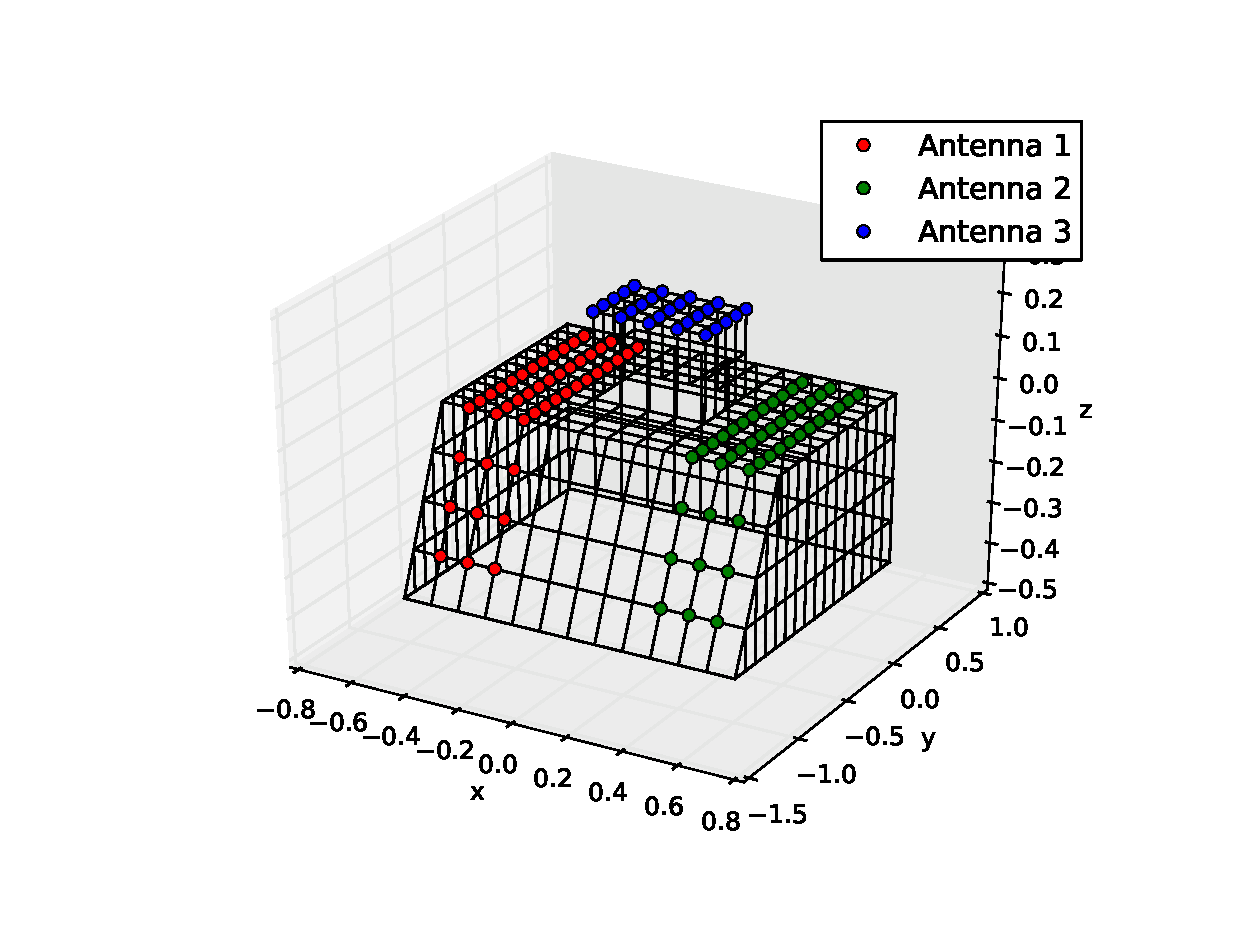
\includegraphics[width=.41\textwidth]{FIG/tc_2_figure}
\end{center}
\caption{Platform used for test case 2 (tc2)}
\label{fig:plat2}
\end{figure}

\begin{figure}
    \begin{center}
        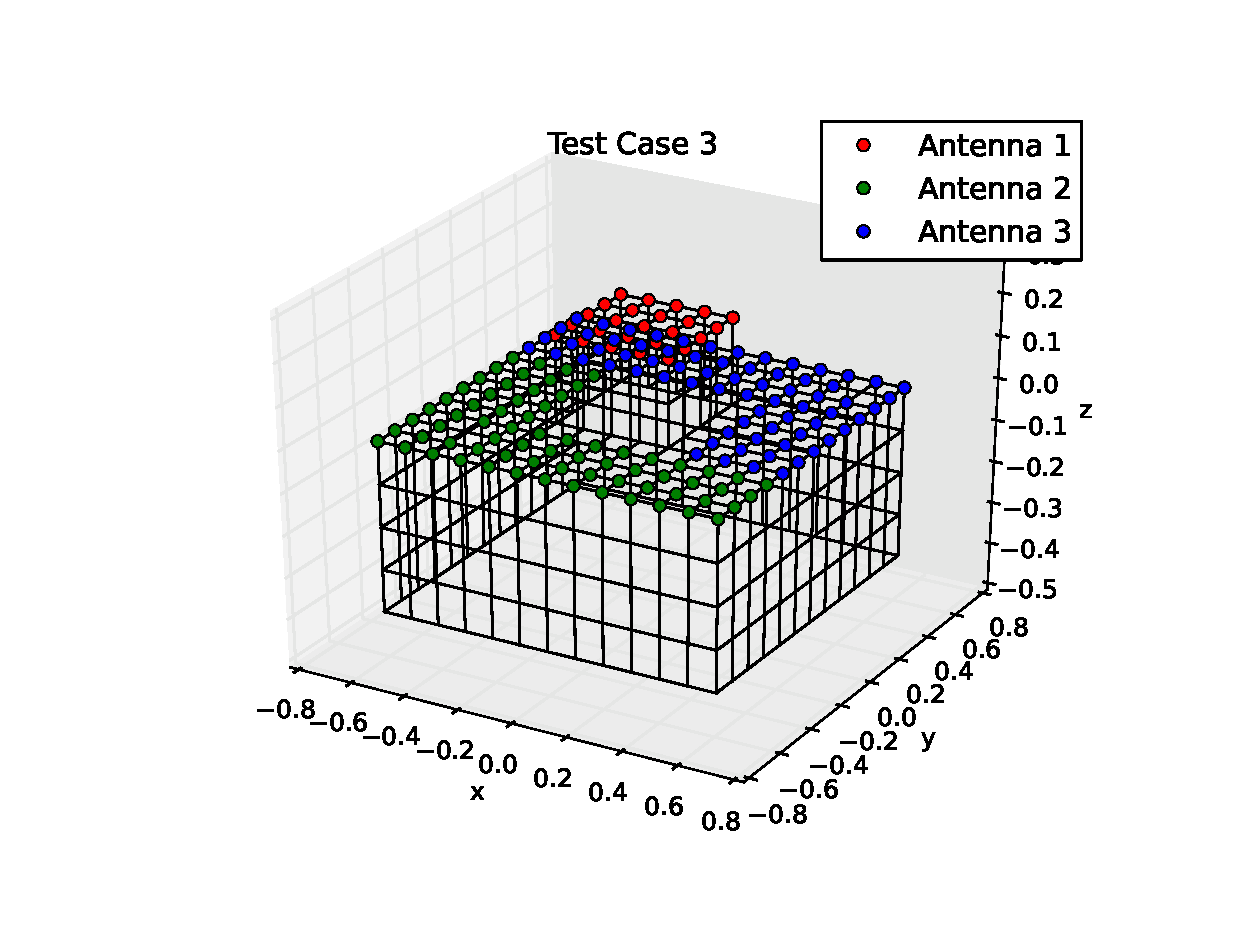
\includegraphics[width=.41\textwidth]{FIG/tc_3_figure}
\end{center}
\caption{Platform used for test case 3 (tc3)}
\label{fig:plat3}
\end{figure}

The number of field points in a radiation pattern is determined by the product of total number of spherical($\theta$) and cylindrical($\phi$) values which encompass points in a sphere. All experiments computed the radiation gain over $4140$ points i.e.$ = \; \mid \theta \mid \cdot \mid \phi \mid$.

For our placement study, $m$ input files would be generated by \textit{EAP} for an hypothesis with $m$ antennas and with only one of the $m$ antennas excited in each input file. Subsequently, NEC would generate $m$ output files with performance measures. By exciting one antenna in each input file, we are able to quantify the radiation pattern of an antenna in presence of the platform and other antennas. To determine the free-space gain pattern(FSG) for an antenna, an input file is formed with just the antenna and no platform. $F_{RP}$ is then calculated by \textit{EAP} parsing $2m$($m$ files with platform and antennas; $m$ files for free space pattern) output files generated by NEC and performing a summation over squared difference in gain between free-space and in the presence of the platform and antennas (Eq.\eqref{eq:rp}).

The second fitness parameter - mutual coupling, is generated by inserting the $CP$ card in the $(m+1)th$ file generated by \textit{EAP} . A single file is needed for NEC to generate an output file with mutual coupling results between all possible pairs of antenna placements of an hypothesis.

All test cases were subjected to the same frequency of $100$ MegaHertz using the $FR$ card. For a detailed description of formatting of $N_{in}$ and $N_{out}$ files, refer to the NEC manual \cite{burke1981numerical}.

\begin{table}
\centering
\caption{Antenna Placement Test Cases} \label{tab:tcs}
\begin{tabular}{|c|c|c|} \hline
    ID&Antennas&Total allowable placements\tablefootnote{Allowable placements for each antenna are provided within parenthesis}\\ \hline
tc1 & 2 & 7,056 (83x83) \\ \hline
tc2 & 3 & 50,625 (45x45x25) \\ \hline
tc3 & 3 & 126,025 (71x71x25) \\ \hline
tc4 & 4 & 20,736 (12x12x12x12) \\
\hline\end{tabular}
\end{table}

\section{Simulation Results}
\label{sec:results}
Comparative study of algorithms is based on multiple test cases listed in Table \ref{tab:tcs}. 

Each test case was first evaluated with an exhaustive search to determine fitness for all allowable placements and antennas. The results from exhaustive search were also used to normalize fitness function values between $[0,1]$. For all experiments $\alpha = \beta = 0.5$ in Eq.\eqref{eq:optimal}. 

Intuitively, a high mutation rate, referred as $p_m$ in Section \ref{sec:algorithms-ga}, drives the algorithm into a random search and renders evolutionary aspect of the algorithm weak. It is preferred to have a high value for $p_c$. For all test cases, \textit{AP-GA} uses $p_m=0.1$ \& $p_c=0.6$. $gen_{max}$ for \textit{AP-GA} and \textit{AP-ES} is $10$.

For similuted annealing, the cooling factor was kept as $1 - \tau$, where $\tau = 0.01 \cdot m_{iters}$. Maximum iterations($m_{iters}$) were about $70\%$ of the total allowable placements of a test case. The initial temperature ranged $\in [0.23, 0.27]$.

The other important observation is of how many number of fitness function evaluations did each algorithm take to find a good hypothesis? Evolutionary strategy and simulated annealing outperformed the genetic algorithm in terms of mean number of fitness evaluations to find the best hypothesis as seen in Table \ref{tab:mean_runs}. The number of evaluations recorded were until the algorithm found the best hypothesis or got stuck at some local optimal hypothesis. Number of function evaluations is more appropriate here rather than the CPU clock time as the time may vary for each machine based on the hardware configuration.

We also visualized the fitness terrain of the best hypothesis followed by each of the stochastic algorithms\footnote{The best hypothesis's fitness curve was almost similar for all 10 runs}. Such visualization is a good tool to observe the correctness of the algorithm. For instance, a simulated annealing is prone to have an event of accepting a bad hypothesis with a higher probability initially in the run and this event should happen with low probability as algorithm proceeds. For all simulated annealing graphs in Figures \ref{fig:tc1}, \ref{fig:tc2}, \ref{fig:tc3}, \& \ref{fig:tc4}, we observe that the gap between any two consecutive events of such nature increases as the algorithm proceeds in the search space. 

The genetic algorithm in Figure \ref{fig:tc2} accepted a worse hypothesis because of the fact that mutation could happen even in the group of elite hypothesis. The elites were included in the mutation pool to maintain diversity. For evolutionary strategy and hill climbing, the fitness terrain does not have unorthodox patterns. The values in parenthesis for all population based algorithms viz. genetic algorithm and evolutionary strategy, represent the population size. They were kept at approximately the same ratio with the corresponding size of the search space in Table \ref{tab:tcs}.

This is not the case, since the top ten hypotheses lie within a small fitness range of $[0.49747, 0.498428]$. As known in general, the hill-climbing algorithm made progress only in the initial phases of the run and got stuck in local optimums for $80\%$ of the runs for test case 3. The purpose for inclusion of such a random search algorithm was to highlight that antenna placements may not be a trivial task to solve with high probability, if the search space is large as in the case of test case $3$. For smaller test cases like test case 4, hill-climbing may be appropriate.

\begin{table*}
\centering
\caption{Mean evaluations}  \label{tab:mean_runs}
\begin{tabular}{|>{\small}c|>{\small}c|>{\small}c|>{\small}c|c|} \hline
\centering
\backslashbox{test case}{method} & AP-GA & AP-ES & AP-SA & AP-HC\\\hline
tc1 & \num{2350} & \num{1728} & \num{667} & \num{164} \\ \hline
tc2 & \num{31680} & \num{11165} & \num{1653} & \num{174} \\ \hline
tc3 & \num{45900} & \num{26880} & \num{4809} & \num{227} \\ \hline
tc4 & \num{6150} & \num{4466} & \num{423} & \num{90} \\ \hline
\end{tabular}
\end{table*}


\begin{figure}
    \begin{center}
        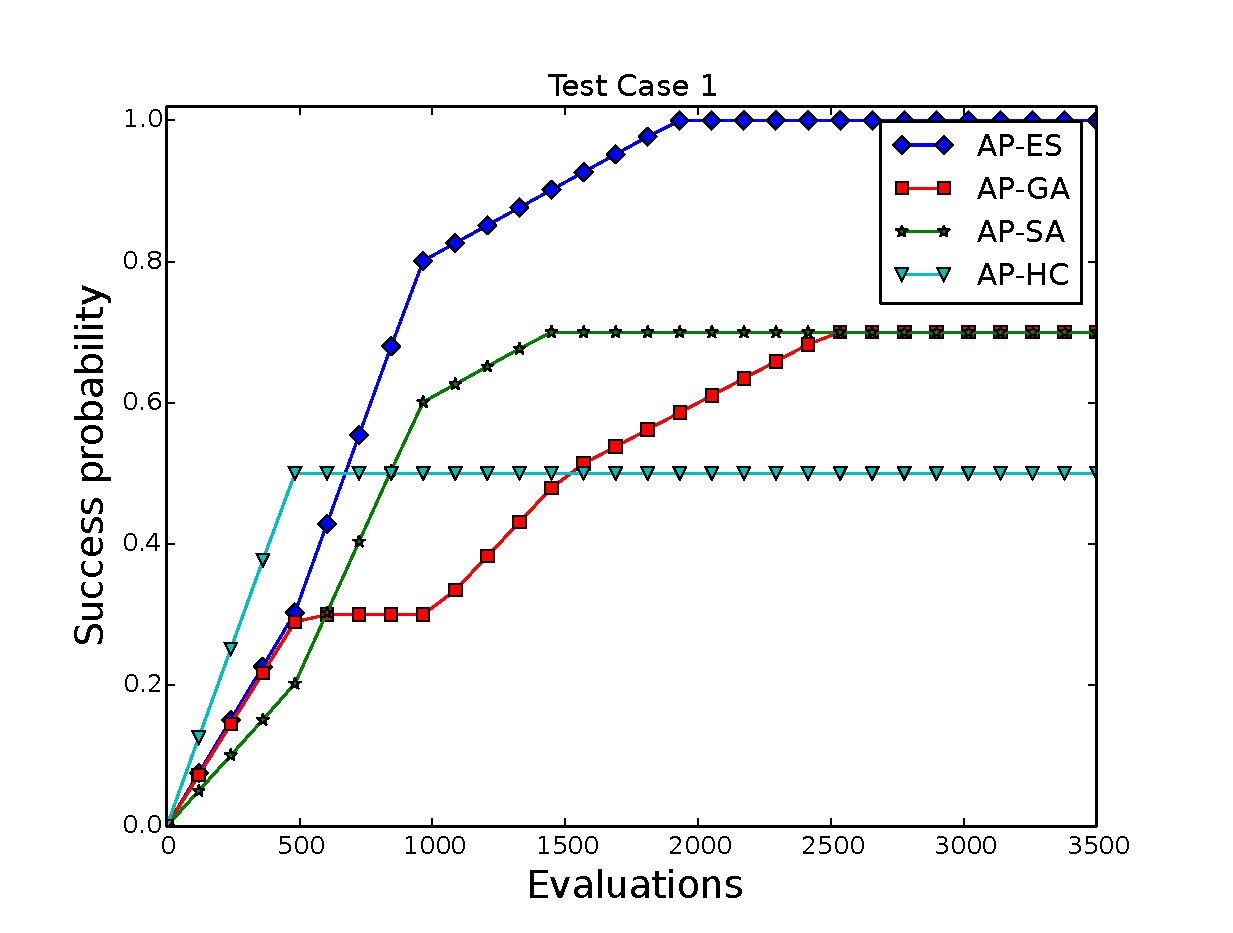
\includegraphics[width=.49\textwidth]{FIG/tc1_sp.eps}
\end{center}
\caption{Test Case 1 Comparison}
\label{fig:tc1}
\end{figure}

\begin{figure}
    \begin{center}
        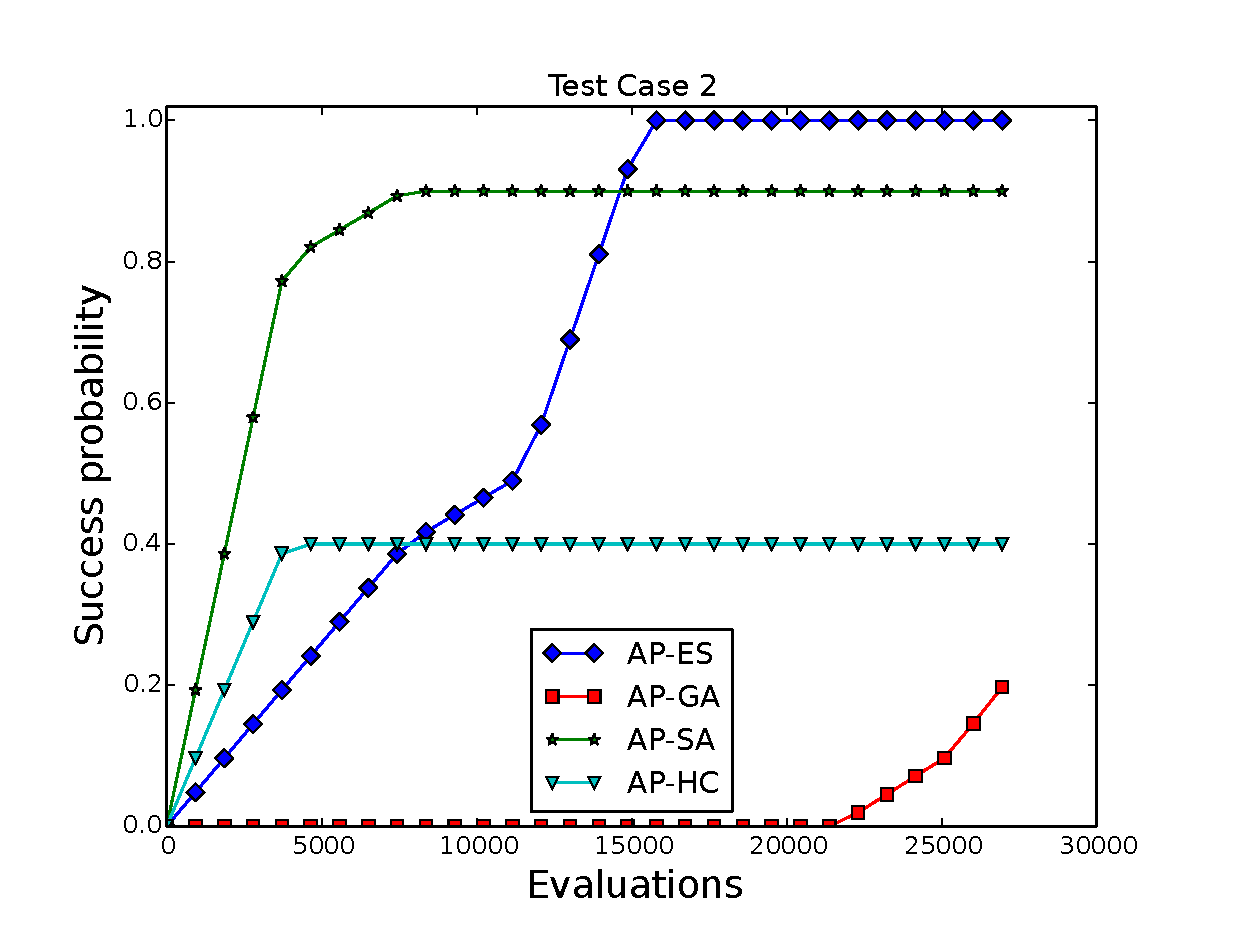
\includegraphics[width=.49\textwidth]{FIG/tc2_sp.eps}
\end{center}
\caption{Test Case 2 Comparison}
\label{fig:tc2}
\end{figure}

\begin{figure}
    \begin{center}
        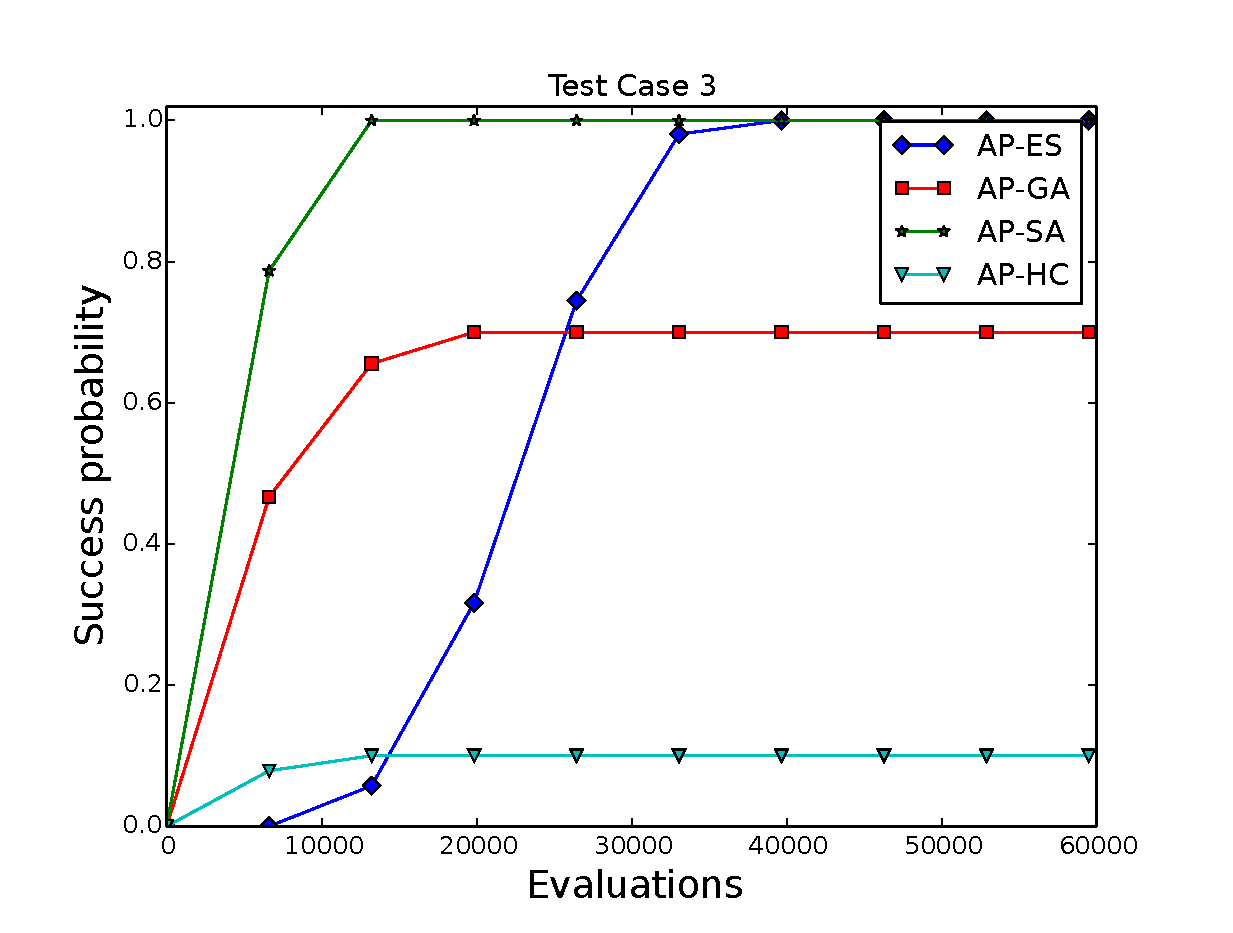
\includegraphics[width=.49\textwidth]{FIG/tc3_sp.eps}
\end{center}
\caption{Test Case 3 Comparison}
\label{fig:tc3}
\end{figure}

\begin{figure}
    \begin{center}
        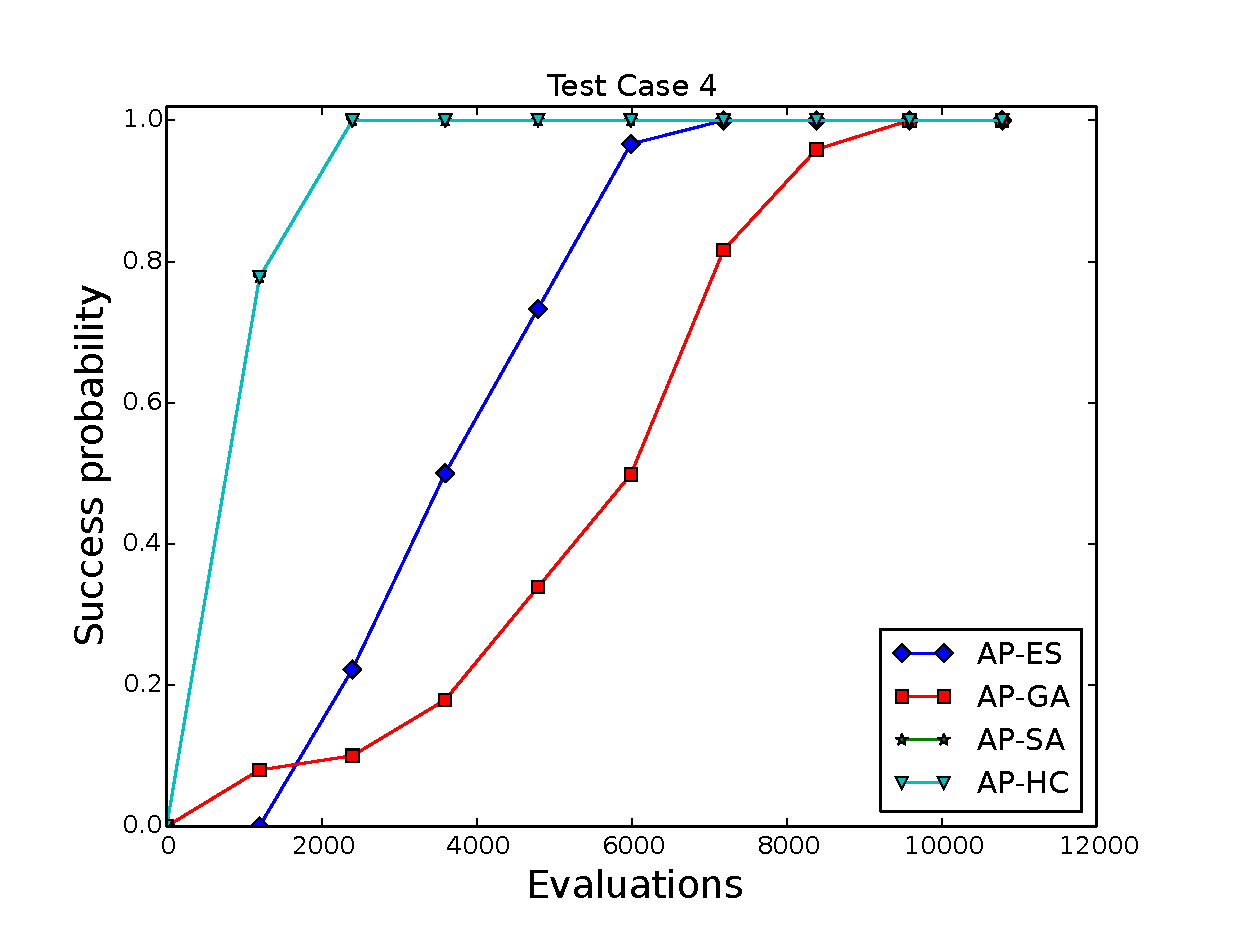
\includegraphics[width=.49\textwidth]{FIG/tc4_sp.eps}
\end{center}
\caption{Test Case 4 Comparison}
\label{fig:tc4}
\end{figure}


\section{Conclusion \& Future Work}
\label{sec-conclusion}
A comparison of four stochastic search algorithms applied to antenna placement optimization was presented. The results showed that a trade-off space exists: faster, less successful simulated annealing (\textit{AP-SA}) search versus slower, more successful search by evolutionary strategy (\textit{AP-ES}). The other generation-based algorithm (\textit{AP-GA}) did not prove as effective as evolutionary strategy, and also much slower to find the optimal placements. Also, a random search was studied to ascertain that the antenna placement problem may not be effectively solved by a greedy algorithm. Moreover, our methodology can be applied to any type of a platform which otherwise may be time consuming and expensive in case of large objects like satellites, warships, and aircrafts. 

Most of the stochastic algorithms presented here were elementary. More experiments need to be conducted for population based algorithms with different population sizes, and to statistically compare how this may affect the performance of the algorithm. Also, bigger search spaces need to be considered with more number of antennas. Other evolutionary techniques like ALPS \cite{hornby2006alps}, and differential evolution algorithm \cite{pan2008discrete} need to be compared for quality and convergence.

\bibliographystyle{plain}
\bibliography{eap_paper} 
\end{document}
